\section{XMD - XMV integration}

\subsection{QML}

The xMAS model designer has been created in QML. QML is a declarative language
that can be used to quickly design user interfaces. It has a JSON-like syntax
which allows developers to describe visual components and their interactions
in a readable and compact notation. Inside a QML file, JavaScript expressions
and functions can be used. This enables developers to add logic using a familiar
scripting language. Furthermore, QML provides a C++ API to connect the user
interface with back-end C++ libraries.

\subsection{User interface}

The applications user interface is composed of multiple qml files. They are split
in two folders. In folder 'uicontrols', the QML files that make up the user interface
controls like the toolbar, console and dialogs are placed. Folder 'xobjects'
contains QML files that are used to draw the xMAS components on the designer
canvas. At the root of the user interface definition is mainWindow.qml.

\paragraph{}
In addition to the qml files, some JavaScript functions are placed in separate
.js files. This has been done for organizational reasons. Small JavaScript fragments
are placed inside the qml files. Larger fragments and fragments that contain logic
are placed inside .js files. This division keeps both files uncluttered. The same
.js file can be imported in multiple qml files, so reuse of code is improved as well.

\subsection{C++ integration}
QML objects can interact with each other by either directly accessing their property
values or through the signal/slot mechanism. Interaction between QML and C++
classes is slightly more complicated. The application uses two methods provided
by QML to integrate QML and C++ objects.

\subsubsection{Context property}
Each QML application operates in a certain QML context. The QML context stores
properties that are available throughout all QML code. C++ classes can be exposed
to the QML world by setting a C++ object instance as the value of a property
on the QML context.
XMD uses context properties to provide access to three C++ classes:

\begin{itemize}
 \item \textbf{datacontrol} (of class DataControl) to provide access to the
 underlying xMAS data model
 \item \textbf{plugincontrol} (of class PluginControl) to provide access to
 the plugins that manage starting and stopping of verification tools
 \item \textbf{util} (of class Util) to provide utility functions
\end{itemize}


%\begin{figure}
%    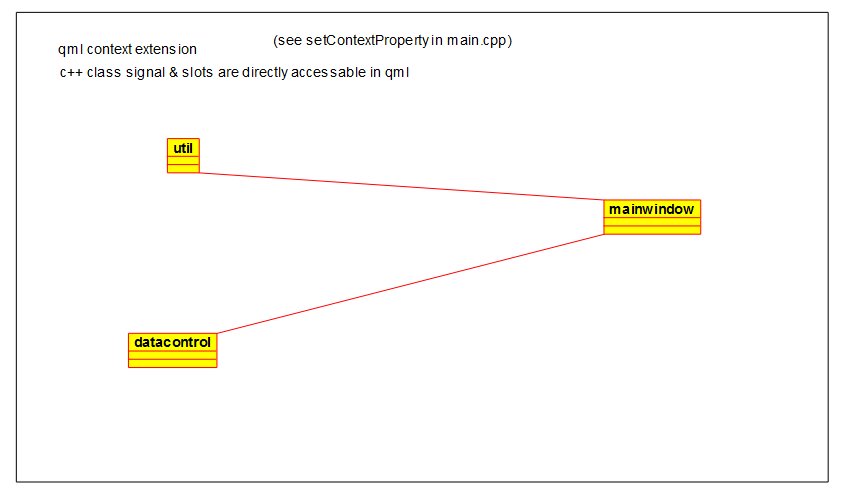
\includegraphics[width=\textwidth]{qml-context-property}
%    \caption{Qml / C++ integration using a context property}
%\end{figure}

More information on context properties is available at:
\url{http://doc.qt.io/qt-5/qtqml-cppintegration-contextproperties.html}


\subsubsection{C++ extension class}

%\begin{figure}
%    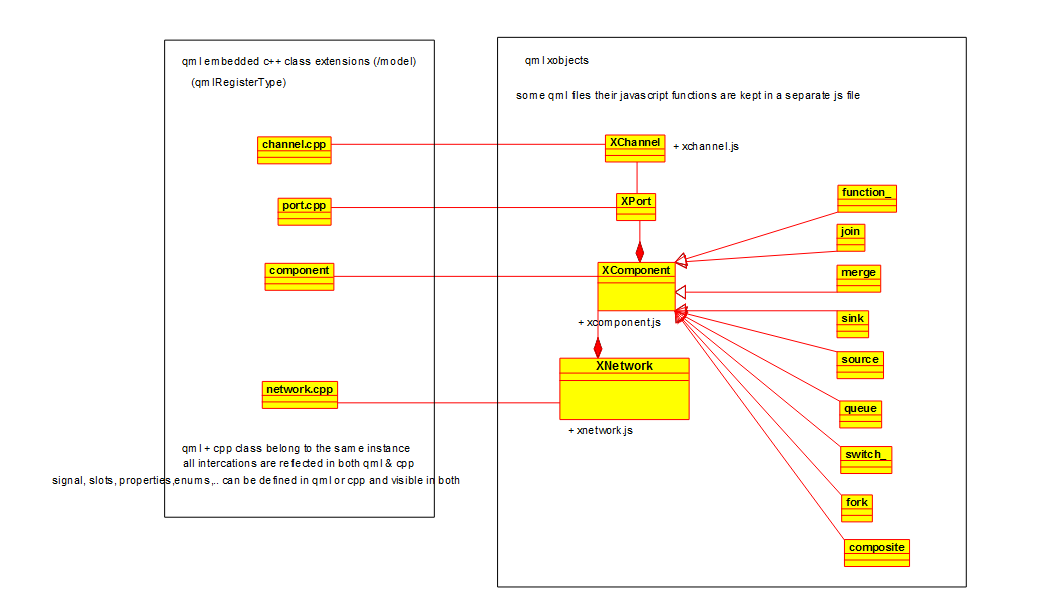
\includegraphics[width=\textwidth]{qml-cpp-extension}
%    \caption{Qml/ C++ integration using an extension class}
%\end{figure}


\subsubsection{Interaction xmd / datamodel classes}

\begin{figure}
    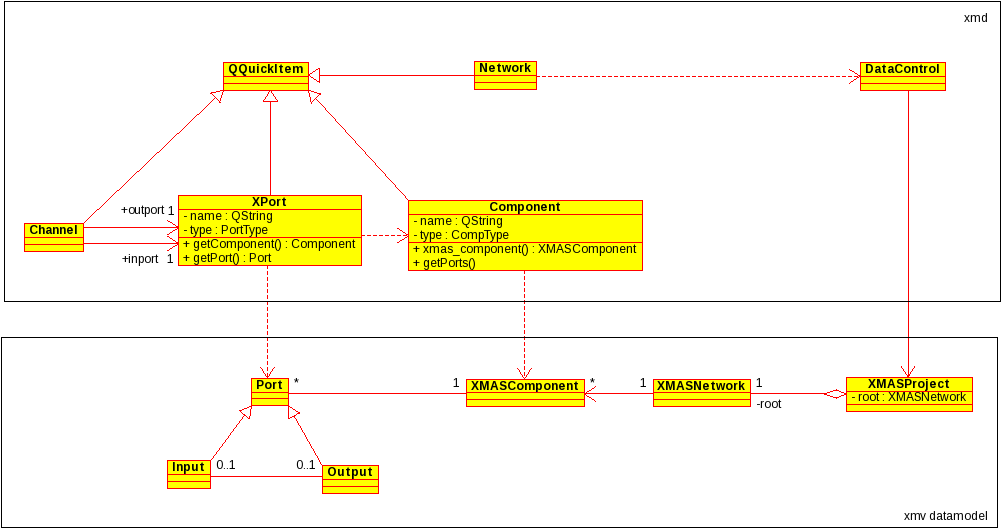
\includegraphics[width=\textwidth]{xmd-xmv-integration}
    \caption{Integration of xmd and xmv datamodel}
\end{figure}
